\section{Haar Wavelet}

\begin{center}
	\begin{minipage}[c]{0.3\textwidth}
		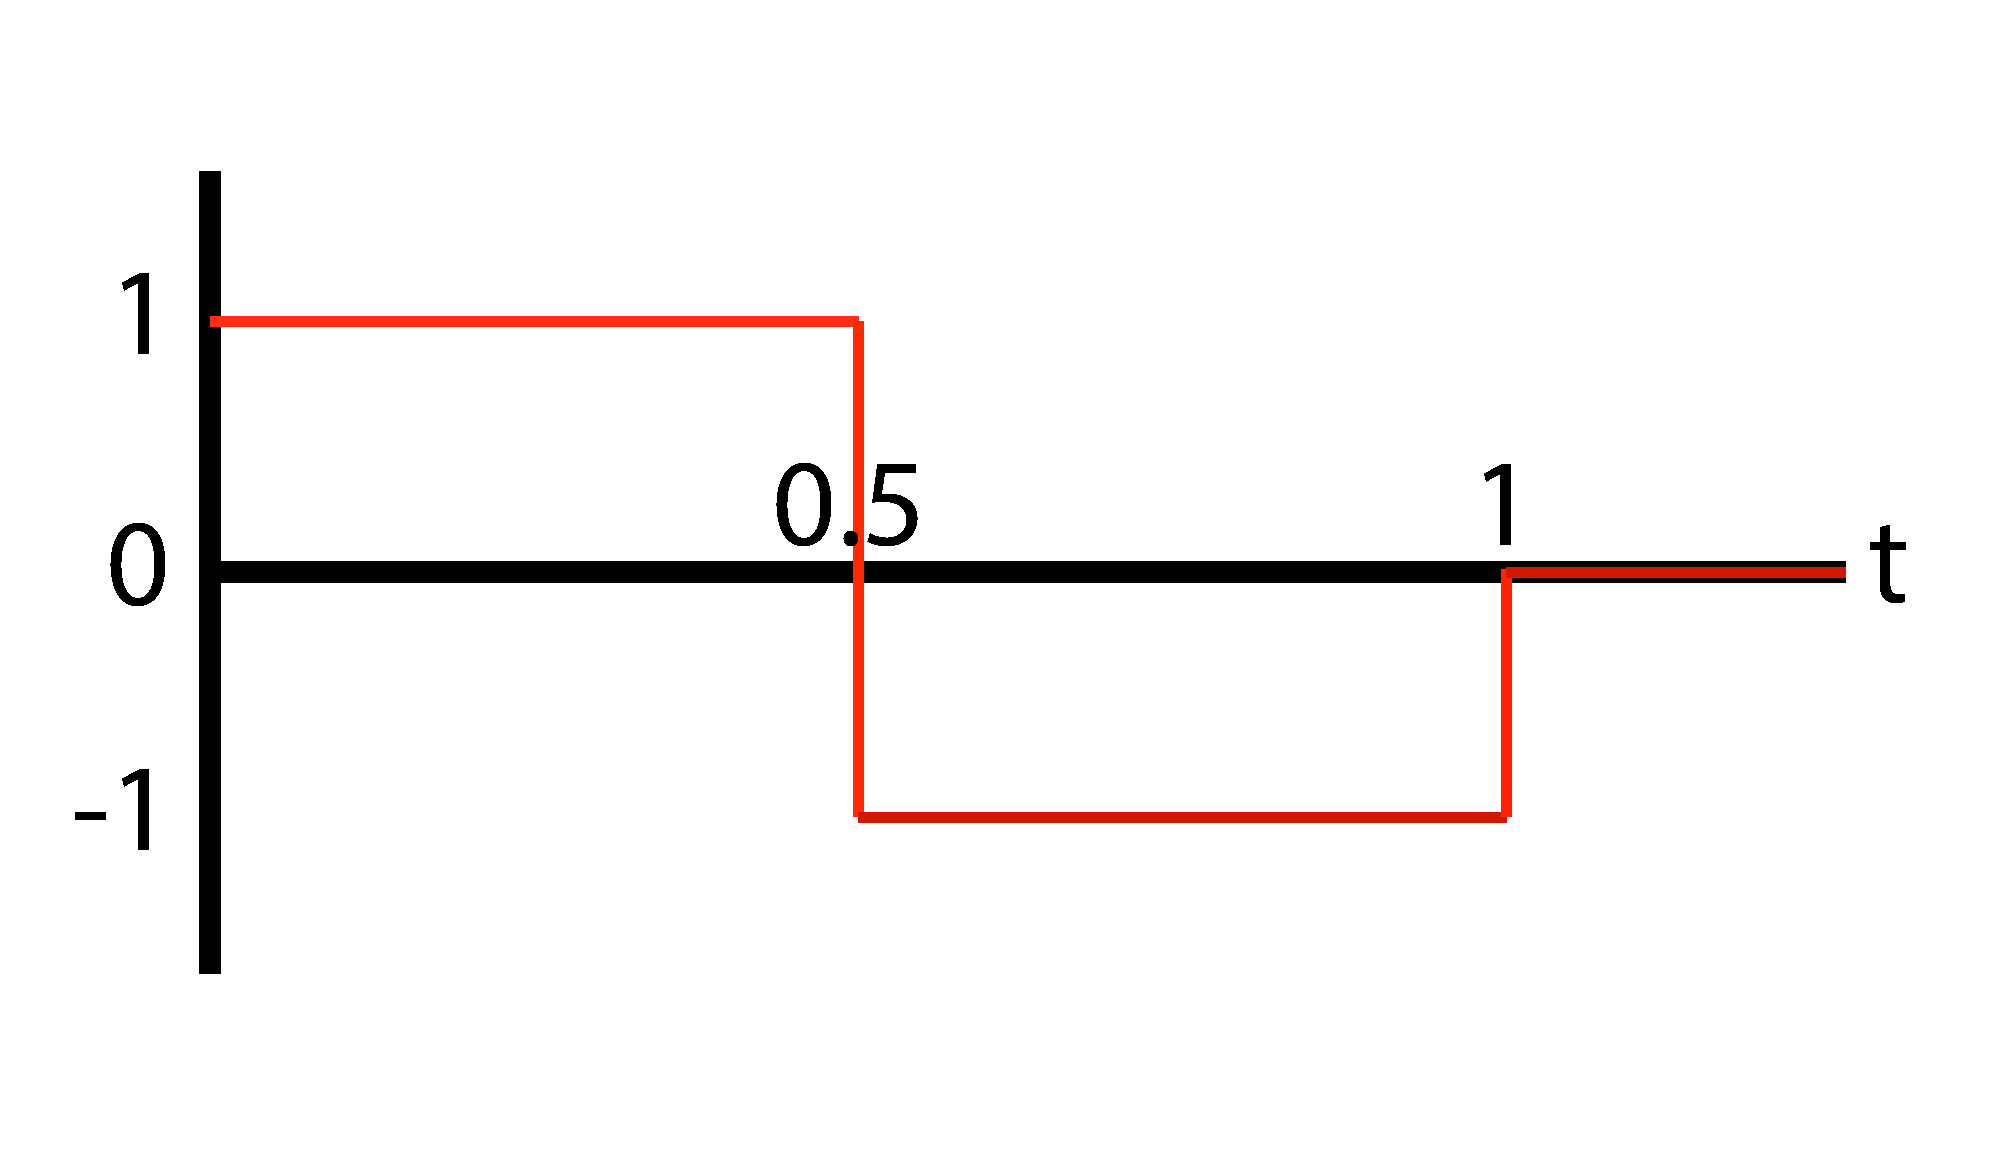
\includegraphics[height=3cm]{content/HaarWavelet.pdf}
	\end{minipage}	
	\begin{minipage}[c]{0.3\textwidth}
		\[
			\psi(t)=\begin{cases} 1 \quad 0 \leq t < \frac{1}{2}\\ -1 \quad \frac{1}{2} \leq t < 1  \end{cases}  
		\]
	\end{minipage}
\end{center}


\[  
	\psi_{m,n}(t)=\frac{1}{\sqrt{2^m}} \cdot \psi(\frac{t}{2^m} - n) = 2^{-m/2} \cdot \psi(2^{-m}t-n) 
	\qquad \qquad
	\psi_{m,n}  = \begin{cases} 
	\frac{1}{\sqrt{2^m}} \qquad 2^m n \leq t < 2^m(n+\frac{1}{2}) \\ 
	\frac{-1}{\sqrt{2^m}} \qquad 2^m(n+\frac{1}{2}) \leq t < 2^m(n+1)
	\end{cases}
\]

\[ 
	\nu_{m,n} = \langle \psi_{m,n} | f \rangle = \int\limits_{-\infty}^{\infty}\psi_{m,n}(t) \cdot f(t) \,\mathrm{d}t = 
	\dfrac{1}{\sqrt{2^m}} \left( \int\limits_{2^mn}^{2^m(\frac12+n)} f(t) \mathrm{d}t - \int\limits_{2^m(\frac12+n)}^{2^m(1+n)}f(t) \mathrm{d}t  \right)
	\quad \Leftrightarrow \quad
	f(t)=\sum_{m,n \in \mathbb{Z}} \nu_{m,n} \cdot \psi_{m,n}
\]

\todo{RK: Übersicht mit Streckungen/Verschiebungen, da geht immer was schief}	
\[  
	||f||^2 = \sum_{m,n \in \mathbb{Z}} |\nu_{m,n}|^2 \qquad \qquad ||f-f_N||^2 = ||f - \sum_{m,n \in \mathbb{Z}}^N \nu_{m,n} \cdot \psi_{m,n}||^2 = \sum_{k=N+1}^{\infty} |c_k|^2
\]
\textbf{TI-89 Haar-Berechnungen}
\begin{alltt}
1/(\(\sqrt{}\)(2^m))*(\(\int\)(f(x),x,2^m*n,2^m*(1/2+n))-\(\int\)(f(x),x,2^m*(1/2+n),2^m*(1+n)))\(\rightarrow\)haar(m,n)
when(0\(\leq\)x,0,when(x<\(\pi\)/2,sin(x),0))\(\rightarrow\)f(x) \(\quad\) when(0\(\leq\)x,0,when(x<1,1,0))\(\rightarrow\)f(x)
haar(m,n)
\end{alltt}

\textbf{Haar-Transformation:}
\begin{enumerate}
	\item Funktion abtasten bei $2^m(n+1/2)$ im Intervall $[a,b] \qquad u_{m,n}\approx \sqrt{2^m}f(2^m[n+1/2])$ 
	\item Die abgetastete Sequenz mit 0 auffüllen bis zu einer Zweierpotenz
	\item In jedem Schritt $u_{m+k+1}, \nu_{m+k+1}$ berechnen
\end{enumerate}

\begin{tabularx}{\textwidth}{p{8cm}|X}
Schnelle Haar-Transformation
  & Schnelle Haar-Rücktransformation\\
$u_{m+1,n} = \dfrac{u_{m,2n}+u_{m,2n+1}}{\sqrt{2}}$
  & $u_{m-1,2n} = \dfrac{u_{m,n}+\nu_{m,n}}{\sqrt{2}}$ \\
$\nu_{m+1,n} = \dfrac{u_{m,2n}-u_{m,2n+1}}{\sqrt{2}}$
  & $\nu_{m-1,2n+1} = \dfrac{u_{m,n}-\nu_{m,n}}{\sqrt{2}}$
\end{tabularx}
